%----------------------------------------------------------------------------
\chapter{Evaluation}
\label{sec:Evaluation}
%----------------------------------------------------------------------------
\providecommand{\miss}{$\times$}

This chapter evaluates the automated rollback platform experimentally. Three detection mechanisms (traffic mirroring, a baseline experiment and a metric-checked canary) are combined in every possible way, a blue-green release is added for comparison, and each of the resulting nine strategies is released with eight versions of the demo application, one healthy and seven faulty. The 72 releases were run, observed and measured by an automated trial runner without manual intervention.

\autoref{sec:EvalQuestions} states the research questions. \autoref{sec:EvalSetup} describes the environment, the faults, the mechanisms and the strategies, and \autoref{sec:EvalRunner} the trial runner and how it measures a release. \autoref{sec:EvalHypotheses} gives the hypotheses, which were written down before the first run. \autoref{sec:EvalResults} presents the results, and \autoref{sec:EvalDeadline} analyses the only result that contradicted the hypotheses: a progress deadline that never fired. \autoref{sec:EvalDiscussion} answers the research questions, and \autoref{sec:EvalThreats} discusses the threats to validity.

%----------------------------------------------------------------------------
\section{Research questions}
\label{sec:EvalQuestions}
%----------------------------------------------------------------------------
The experiments answer five questions.

\begin{description}
	\item[RQ1] Which detection mechanism catches which kind of fault, and how fast?
	\item[RQ2] What does each strategy cost, in users exposed to a faulty version and in the time and resources of a healthy release?
	\item[RQ3] How do absolute checks (fixed thresholds on the new version alone) compare with relative checks (the new version compared with a fresh copy of the old one)?
	\item[RQ4] Do combined mechanisms protect better than single ones, and which combinations only add time?
	\item[RQ5] What changes when the gradual canary is replaced by an all-at-once blue-green switch?
\end{description}

The scope is limited to faults \emph{in the release itself}: the new version is faulty, while the cluster, the network and the dependencies are healthy. Environment faults, such as a node under CPU pressure, are left for future work (\autoref{sec:EvalThreats}).

%----------------------------------------------------------------------------
\section{Experimental setup}
\label{sec:EvalSetup}
%----------------------------------------------------------------------------

%----------------------------------------------------------------------------
\subsection{Environment and load}
\label{sec:EvalEnvironment}
%----------------------------------------------------------------------------
All runs used the development environment of the platform: a single-node k3s cluster with Istio as the service mesh, Prometheus as the metric store, Argo Rollouts v1.10.1 as the release controller and Argo CD as the GitOps agent~\cite{ArgoCD}. Every change to an application, including the image tag that triggers a release, is a commit in the platform's Git repository, which Argo CD applies to the cluster.

The demo application is a small HTTP service with one replica per version. A load generator inside the cluster sends a request to \texttt{GET /api/work} every 0.2\,s through the Istio ingress gateway, about 5 requests per second in total, at the same rate in every run. Prometheus scrapes the Envoy sidecars every 10\,s. Because a single request is usually not measured on its own, every time below is only accurate to about 10--20\,s.

%----------------------------------------------------------------------------
\subsection{Fault injection}
\label{sec:EvalFaults}
%----------------------------------------------------------------------------
Each fault is a separate image of the demo application, built by the CI pipeline from the same source commit with a different build setting (\autoref{tab:EvalFaults}). A fault is therefore part of the version being released, and it is present from the first request on, exactly as a bug shipped in a release would be. The faults were chosen to cover different kinds of failure: loud and fast (F1, F3), below a threshold (F2), noisy (F4), slow-burning (F5), failing at start-up (F6) and semantic, invisible to request metrics (F8). F0 is the healthy control, used to detect false alarms and to measure the cost of a release that should simply succeed.

\begin{table}[ht]
	\footnotesize
	\centering
	\begin{tabular}{ l l l l }
		\toprule
		ID & Fault & Build setting & Kind \\
		\midrule
		F0 & healthy version & none & control \\
		F1 & 30\,\% of requests return HTTP 500 & \texttt{ERROR\_RATE=30} & loud, fast \\
		F2 & 2\,\% of requests return HTTP 500 & \texttt{ERROR\_RATE=2} & below every threshold \\
		F3 & every response delayed by 800\,ms & \texttt{LATENCY\_MS=800} & loud, fast \\
		F4 & random delay of 0--1500\,ms & \texttt{LATENCY\_JITTER\_MS=1500} & noisy tail latency \\
		F5 & memory grows by 20\,MiB per minute & \texttt{LEAK\_MB\_PER\_MIN=20} & slow-burn \\
		F6 & readiness probe always fails & \texttt{FAIL\_READINESS=true} & start-up \\
		F8 & wrong result with HTTP 200 & \texttt{WRONG\_ANSWER=true} & semantic \\
		\bottomrule
	\end{tabular}
	\caption{Injected faults. Each is a separate image built from the same source commit. (F7, an environment fault, was dropped from the scope; its identifier was kept free.)}
	\label{tab:EvalFaults}
\end{table}

%----------------------------------------------------------------------------
\subsection{Detection mechanisms}
\label{sec:EvalMechanisms}
%----------------------------------------------------------------------------
Three mechanisms can protect a canary release, and each can be switched on or off independently. When several are on, they always run in the same order, mirroring first, then the experiment, then the canary steps.

\paragraph{M -- traffic mirroring.} The new version is scaled to one pod while it receives no user traffic, and Istio copies every \texttt{GET /api/work} request to it~\cite{IstioVirtualService}. The responses of the copy are discarded, so no user ever sees them. During mirroring, the AnalysisTemplate \texttt{mirror-health} takes three measurements 20\,s apart, after a 30\,s initial delay. It measures the success rate (at least 95\,\%, no failed measurement allowed) and the 95th percentile latency (at most 300\,ms, one failure allowed) of the requests the new pods received. It has no memory check, because mirroring lasts only about 70\,s.

\paragraph{E -- baseline experiment.} An Argo Rollouts \emph{experiment} step starts two fresh pods side by side for three minutes, a \emph{baseline} running the stable version and a \emph{canary} running the new one, and sends 20\,\% of the users to each~\cite{ArgoRolloutsExperiment}. The AnalysisTemplate \texttt{canary-vs-baseline} compares the two every 20\,s: the canary's 5xx ratio may exceed the baseline's by at most 5 percentage points, its p95 latency by at most 100\,ms, and its memory growth by at most 0.05\,MiB/s. Because both pods start at the same moment, effects of start-up, such as the initial memory allocation, cancel out in the difference. This makes E the only \emph{relative} check of the platform.

\paragraph{C -- canary steps.} The canary receives 10\,\% of the users for one minute, then 50\,\% for one minute, before being promoted. A background analysis, \texttt{canary-health}, runs during these steps and checks the success rate (at least 95\,\%) and the p95 latency (at most 300\,ms) every 30\,s, with one failure allowed, and the memory growth (at most 0.05\,MiB/s) every 30\,s after a 90\,s delay, with no failure allowed. These are \emph{absolute} thresholds, applied to the new version on its own.

\paragraph{BG -- blue-green with a smoke test.} The blue-green variant of the demo application uses a separate Rollout with an active and a preview Service~\cite{ArgoRolloutsBlueGreen}. The new version first starts behind the preview Service, which receives no user traffic. A pre-promotion analysis then runs a Kubernetes Job~\cite{ArgoRolloutsJob}, which sends 50 requests to the preview Service and fails if any of them returns an error or an incorrect result. Only then are all users switched to the new version at once. A post-promotion analysis, \texttt{bg-post-promotion}, then checks the success rate, the p95 latency and the memory growth of the now active version for about two and a half minutes, and aborts the release (switching the users back) if they fail. The Job runs inside the mesh under strict mutual TLS, which requires the native sidecar mode of Kubernetes, so that the Envoy proxy starts before the test and stops after it~\cite{K8sSidecar}.

\paragraph{The progress deadline.} Independently of the strategy, every Rollout sets \texttt{progressDeadlineSeconds: 120} and \texttt{progressDeadlineAbort: true}~\cite{ArgoRolloutsSpec}. If a release makes no progress for 120\,s, for example because its pods never become Ready, the controller should abort it. This is a property of the Rollout, not a step, so it is part of every strategy including the control.

%----------------------------------------------------------------------------
\subsection{Strategies}
\label{sec:EvalStrategies}
%----------------------------------------------------------------------------
The three canary mechanisms were combined in a full factorial design~\cite{Montgomery17}: each of M, E and C is either on or off, which gives the eight strategies S0--S7 of \autoref{tab:EvalStrategies}, plus the blue-green strategy BG. The single-mechanism strategies S1--S3 show what each mechanism catches on its own, while S4--S7 show whether a combination catches more, or only takes longer.

A release must end at 100\,\%: when the last step finishes, the Rollout promotes the new version. A strategy without C therefore sends all users to the new version right after its last check, and a fault that this check missed reaches everyone. This is the honest standalone behaviour of the mechanism, and the reason why S2 and S3 are not merely shorter versions of S7. S0, with no steps at all, is the control: it releases the new version to all users at once, protected only by the progress deadline.

\begin{table}[ht]
	\footnotesize
	\centering
	\begin{tabular}{ l c c c l }
		\toprule
		ID & M & E & C & Meaning \\
		\midrule
		S0 & & & & control: no progressive delivery, only the progress deadline \\
		S1 & & & \checkmark & canary alone \\
		S2 & \checkmark & & & mirroring alone \\
		S3 & & \checkmark & & experiment alone \\
		S4 & \checkmark & & \checkmark & mirroring, then canary \\
		S5 & & \checkmark & \checkmark & experiment, then canary \\
		S6 & \checkmark & \checkmark & & mirroring, then experiment \\
		S7 & \checkmark & \checkmark & \checkmark & all three (the platform's default configuration) \\
		BG & & & & blue-green: preview, smoke Job, switch, post-promotion analysis \\
		\bottomrule
	\end{tabular}
	\caption{The strategies under test. M: mirroring, E: baseline experiment, C: canary steps.}
	\label{tab:EvalStrategies}
\end{table}

The parameters of each mechanism (durations, weights, intervals and thresholds) are the same in every strategy, so any difference between two strategies comes only from the mechanisms that differ between them. The strategies are implemented as Kustomize components~\cite{KustomizeComponents}, one per strategy, each of which replaces the steps of the default Rollout (S7). The component \texttt{s7-all} is empty, so the default configuration is tested exactly as it is deployed. A script generates the components from shared blocks, which guarantees that the M, E and C steps are byte-for-byte identical wherever they appear. Switching the strategy changes a single line of the development overlay.

%----------------------------------------------------------------------------
\section{Trial automation}
\label{sec:EvalRunner}
%----------------------------------------------------------------------------
Running 72 releases by hand, with a clock and a dashboard, would be slow and, worse, inconsistent. The trial runner, a Python program using only the standard library, performs every run in the same way and records what happened in enough detail to recompute every measurement later.

%----------------------------------------------------------------------------
\subsection{A trial as a sequence of commits}
\label{sec:EvalTrial}
%----------------------------------------------------------------------------
Because Argo CD reverts any change made to the cluster directly, the runner changes the platform the same way a developer would: through Git. A trial consists of the following steps.
\begin{enumerate}
	\item \textbf{Preconditions.} The other application must not be releasing, and the application under test must be Healthy on its reset tag, a healthy image. Otherwise the runner resets it first.
	\item \textbf{Strategy.} If the strategy differs from the current one, the runner edits the component line of the overlay, commits, pushes, asks Argo CD to refresh, and waits until Argo CD reports this commit as synced.
	\item \textbf{Trigger.} Once the observer has recorded the initial state, the runner commits the image tag of the fault under test. This commit starts the release.
	\item \textbf{Observation.} The runner follows the release until it is promoted, or until it is aborted and no user traffic reaches the new version for 10\,s. If neither happens within 20 minutes (4 minutes for F6), it records a timeout and aborts the release itself.
	\item \textbf{Measurement.} The timeline and Prometheus are turned into measurements, which are saved as one row of a CSV file and, together with the raw timeline, as a JSON record.
	\item \textbf{Reset.} The runner commits the reset tag. After an abort this is instant, since the stable version is already running. After a promotion the faulty version has become stable, so the reset is itself a release; it runs under S0 to take seconds instead of minutes. A 60\,s pause then separates the trial from the next one, so that the one-minute rate windows of the queries do not overlap.
\end{enumerate}
Every trial is thus traceable to the commits that defined its strategy and triggered its release. The runner groups the trials by strategy to minimise switches, and skips trials that already have a result, so an interrupted matrix can be resumed.

%----------------------------------------------------------------------------
\subsection{Observation}
\label{sec:EvalObservation}
%----------------------------------------------------------------------------
Every two seconds, the runner reads the Rollout, its AnalysisRuns and Experiments, the VirtualService, the Services and the pods of the application in a single \texttt{kubectl} call, and reduces them to a small \emph{snapshot}: the phase, step and abort flag of the Rollout, the current and stable pod-template hashes, the route weights and the mirror target, the phase and failure count of each metric of the new version, and the pods. A snapshot is stored only when it differs from the previous one, so the \emph{timeline} of a trial is the list of its state changes, each with a timestamp.

Where users go is read from the routing objects themselves, not from the Rollout's status, because these are what actually route the traffic. For a canary, this is the weight of the canary destinations in the VirtualService; for blue-green, the pod-template hash selected by the active Service. Once the new version is promoted, the stable Service points to it, so it serves 100\,\% of the users.

%----------------------------------------------------------------------------
\subsection{Measurements}
\label{sec:EvalMeasurements}
%----------------------------------------------------------------------------
\autoref{tab:EvalMeasurements} defines the measurements. Times come from the timeline. The moment of detection is the \texttt{finishedAt} time of the first failing measurement, recorded by the controller in cluster time and converted with the clock offset between the cluster and the runner, which the runner measures at the start of each trial.

\begin{table}[ht]
	\footnotesize
	\centering
	\begin{tabular}{ l p{11cm} }
		\toprule
		Measurement & Definition \\
		\midrule
		outcome & \emph{promoted}, \emph{aborted}, or \emph{timeout} if the release did not end by itself \\
		caught by & the check whose failing measurement finished first, or the progress deadline \\
		TTD & time to detect: from the first request of any kind to the new version (a mirrored copy, a user request or a smoke-test request) until detection \\
		TTR & time to recover: from detection until no user and no mirrored request reaches the new version \\
		max.\ exposure & the highest share of users routed to the new version \\
		user requests & requests the ingress gateway sent to the new version, counted at the new pods' sidecars; of these, \emph{affected} are those answered with a 5xx code or slower than 500\,ms \\
		duration & for a promoted release: from the start until the promotion \\
		pod-minutes & the summed lifetime of the pods created during the trial \\
		\bottomrule
	\end{tabular}
	\caption{Measurements recorded for every trial.}
	\label{tab:EvalMeasurements}
\end{table}

Request counts come from the Istio standard metrics \texttt{istio\_requests\_total} and \texttt{istio\_request\_duration\_milliseconds}~\cite{IstioMetrics}, reported by the sidecars of the new version and selected by its pod-template hash, so that every route to it is counted, including the stable Service after a promotion. The experiment's canary pod has its own hash, so it is counted through its own Service. Mirrored copies also come from the gateway, so the user window starts only when mirroring has ended. Mirrored copies and smoke-test requests are counted separately. The threshold for a slow request is 500\,ms rather than the 300\,ms of the latency checks, because Istio's histogram has no bucket between 250 and 500\,ms~\cite{PromHistograms}.

\paragraph{Exact counting.} The usual way to count requests in a window, PromQL's \texttt{increase()}, extrapolates the counter to the edges of the window~\cite{PromQL}. For short bursts this overcounts considerably: in a validation run, it reported 63 smoke-test requests where the Job's log showed exactly 50. The runner therefore takes the last value of each counter series up to the end of the window and subtracts its last value before the start, treating a series that did not exist yet as zero. With this method the same run gives exactly 50. The windows end 30\,s after the event that closes them, to include the final scrape.

\paragraph{Validation.} Before the matrix, the runner was validated on a recorded blue-green release (promoted, 50 smoke requests, no errors), on a synthetic aborted canary with mirroring, and on a live faulty blue-green release. These runs revealed two defects, which were fixed before the matrix: snapshots taken before the release started still showed the analysis runs of the previous release, and the recorded Git commit did not yet include the trigger. The matrix itself revealed four more, all in the measurement code and none in the observation, so the stored timelines were re-measured afterwards: promoted releases were reported with 0\,\% exposure, their user requests were undercounted, progress-deadline aborts were labelled with the raw controller message, and pods that appeared in a single snapshot were counted with zero lifetime.

%----------------------------------------------------------------------------
\section{Hypotheses}
\label{sec:EvalHypotheses}
%----------------------------------------------------------------------------
Before the first run, the expected result of every cell was written down from the configuration alone (\autoref{tab:EvalHypotheses}). With combined mechanisms, the first one in the order M, E, C that catches a fault should decide the outcome, and the later ones should never run. Some predictions follow directly from the design:
\begin{itemize}
	\item F2 should pass every metric check, since 2\,\% errors is below both the 95\,\% success threshold and the 5-point delta. Blue-green should catch it only by chance: 50 requests all succeed with probability $0.98^{50} \approx 36\,\%$, so the Job fails in about 64\,\% of the runs.
	\item F8 returns correct HTTP status codes with a wrong body, so only the smoke Job, which checks the body, should catch it.
	\item Mirroring has no memory check and lasts about 70\,s, so it should let F5 through to all users (S2), or pass it on to the next mechanism (S4, S6, S7).
	\item The canary's memory check starts after 90\,s, when the canary is already at 50\,\%, so C should catch F5 at 50\,\% exposure.
	\item Placing E before C should make the loud faults \emph{worse} than C alone, because E exposes 20\,\% of the users while the canary's first step exposes only 10\,\%.
	\item F6 never becomes Ready and therefore never receives any traffic, so in every strategy it should be stopped by the progress deadline after about 120\,s, with no user exposed.
\end{itemize}

\begin{table}[ht]
	\scriptsize
	\centering
	\setlength{\tabcolsep}{3pt}
	\begin{tabular}{ l c c c c c c c c }
		\toprule
		& F0 & F1 & F2 & F3 & F4 & F5 & F6 & F8 \\
		\midrule
		\textbf{S0} & pass & \miss & \miss & \miss & \miss & \miss & DL · 0\,\% & \miss \\
		\textbf{S1} C & pass & C · 10\,\% & \miss & C · 10\,\% & C · 10\,\% & C · 50\,\% & DL · 0\,\% & \miss \\
		\textbf{S2} M & pass & M · 0\,\% & \miss & M · 0\,\% & M · 0\,\% & \miss & DL · 0\,\% & \miss \\
		\textbf{S3} E & pass & E · 20\,\% & \miss & E · 20\,\% & E · 20\,\% & E · 20\,\% & DL · 0\,\% & \miss \\
		\textbf{S4} M+C & pass & M · 0\,\% & \miss & M · 0\,\% & M · 0\,\% & C · 50\,\% & DL · 0\,\% & \miss \\
		\textbf{S5} E+C & pass & E · 20\,\% & \miss & E · 20\,\% & E · 20\,\% & E · 20\,\% & DL · 0\,\% & \miss \\
		\textbf{S6} M+E & pass & M · 0\,\% & \miss & M · 0\,\% & M · 0\,\% & E · 20\,\% & DL · 0\,\% & \miss \\
		\textbf{S7} M+E+C & pass & M · 0\,\% & \miss & M · 0\,\% & M · 0\,\% & E · 20\,\% & DL · 0\,\% & \miss \\
		\textbf{BG} & pass & Job · 0\,\% & Job (64\,\%) & post · 100\,\% & post · 100\,\% & post · 100\,\% & DL · 0\,\% & Job · 0\,\% \\
		\bottomrule
	\end{tabular}
	\caption{Hypotheses, written before the first run: the check expected to stop the release, and the highest share of users exposed. \miss: not caught, the faulty version reaches all users. DL: progress deadline. Job: pre-promotion smoke test. post: post-promotion analysis. pass: the healthy version was promoted, as it should be.}
	\label{tab:EvalHypotheses}
\end{table}

%----------------------------------------------------------------------------
\section{Results}
\label{sec:EvalResults}
%----------------------------------------------------------------------------
The 72 trials ran unattended on 1 November 2026 between 13:15 and 17:35, in 4 hours and 20 minutes, 3.6 minutes per trial on average including the resets and pauses. Every trial completed; none had to be repeated.

%----------------------------------------------------------------------------
\subsection{Detection}
\label{sec:EvalDetection}
%----------------------------------------------------------------------------
\autoref{tab:EvalDetection} shows what stopped each release and the highest share of users exposed to it. \textbf{70 of the 72 cells match the hypotheses.} The two exceptions are S6 and S7 with F6, where the progress deadline did not fire, and the release stayed at its first step until the runner aborted it after four minutes. \autoref{sec:EvalDeadline} analyses these two cells. In both, no user was exposed, since the new version never became Ready.

\begin{table}[ht]
	\scriptsize
	\centering
	\setlength{\tabcolsep}{3pt}
	\begin{tabular}{ l c c c c c c c c }
		\toprule
		& F0 & F1 & F2 & F3 & F4 & F5 & F6 & F8 \\
		\midrule
		\textbf{S0} & pass & \miss & \miss & \miss & \miss & \miss & DL · 0\,\% & \miss \\
		\textbf{S1} C & pass & C · 10\,\% & \miss & C · 10\,\% & C · 10\,\% & C · 50\,\% & DL · 0\,\% & \miss \\
		\textbf{S2} M & pass & M · 0\,\% & \miss & M · 0\,\% & M · 0\,\% & \miss & DL · 0\,\% & \miss \\
		\textbf{S3} E & pass & E · 20\,\% & \miss & E · 20\,\% & E · 20\,\% & E · 20\,\% & DL\textsubscript{E} · 0\,\% & \miss \\
		\textbf{S4} M+C & pass & M · 0\,\% & \miss & M · 0\,\% & M · 0\,\% & C · 50\,\% & DL · 0\,\% & \miss \\
		\textbf{S5} E+C & pass & E · 20\,\% & \miss & E · 20\,\% & E · 20\,\% & E · 20\,\% & DL\textsubscript{E} · 0\,\% & \miss \\
		\textbf{S6} M+E & pass & M · 0\,\% & \miss & M · 0\,\% & M · 0\,\% & E · 20\,\% & \textbf{hang} · 0\,\% & \miss \\
		\textbf{S7} M+E+C & pass & M · 0\,\% & \miss & M · 0\,\% & M · 0\,\% & E · 20\,\% & \textbf{hang} · 0\,\% & \miss \\
		\textbf{BG} & pass & Job · 0\,\% & Job · 0\,\% & post · 100\,\% & post · 100\,\% & post · 100\,\% & DL · 0\,\% & Job · 0\,\% \\
		\bottomrule
	\end{tabular}
	\caption{Measured results: the check that stopped the release, and the highest share of users exposed. DL\textsubscript{E}: the experiment's own progress deadline. hang: no check stopped the release. Other symbols as in \autoref{tab:EvalHypotheses}.}
	\label{tab:EvalDetection}
\end{table}

Some cells match the hypotheses in a way worth noting:
\begin{itemize}
	\item \textbf{No false alarms.} All nine healthy releases (F0) were promoted.
	\item \textbf{F6 under S3 and S5} was stopped by the deadline of the experiment, not of the Rollout. These strategies start with the experiment step, whose canary template has its own progress deadline; it expired after 120\,s and failed the experiment, which aborted the Rollout. The outcome is the same as predicted.
	\item \textbf{F2 under BG} was caught: one of the 50 smoke requests failed. This is the more likely of the two possible outcomes (about 64\,\%). A single run cannot show the rate.
	\item \textbf{F5 under S4, S6 and S7} passed mirroring, as predicted, and was caught by the next mechanism: by the canary at 50\,\% in S4, and by the experiment at 20\,\% in S6 and S7.
	\item \textbf{F8} was caught only by the smoke Job's body check; every canary strategy promoted it.
\end{itemize}

%----------------------------------------------------------------------------
\subsection{Time to detect and to recover}
\label{sec:EvalTTD}
%----------------------------------------------------------------------------
\autoref{tab:EvalTTD} lists the time to detect. Each mechanism has a characteristic detection time, set mainly by its initial delay, its interval and the number of failures it tolerates, and much less by the fault:
\begin{itemize}
	\item Mirroring catches F1 in 27--29\,s: its success-rate metric tolerates no failure, so the first measurement after the 30\,s delay decides. It catches latency in 47--49\,s, because the latency metric tolerates one failure, so the second measurement decides.
	\item The experiment catches errors and latency in 47--51\,s (one failure allowed, 20\,s interval) and the leak in 57--61\,s.
	\item The canary catches errors and latency in 57--59\,s (one failure allowed, 30\,s interval) and the leak in 87\,s.
	\item The smoke Job catches F1, F2 and F8 in 15--17\,s, the time needed to start the Job and send 50 requests.
	\item The post-promotion analysis catches F3--F5 in 82--111\,s, all of it with every user on the faulty version.
\end{itemize}
The run-to-run differences between faults caught by the same check were within one measurement interval. Noisy latency (F4) was caught as quickly as constant latency (F3), contrary to the expectation that it would be slower and more variable: a random delay of up to 1500\,ms puts the p95 at about 1400\,ms, far above the 300\,ms threshold.

For F5 under S4, S6 and S7, the time to detect (139--170\,s) is long only because it counts from the first mirrored request: the leak went unnoticed during mirroring and was caught by the next mechanism. Measured from the start of the experiment or the canary step, it is the same as under S3 or S1.

\begin{table}[ht]
	\footnotesize
	\centering
	\begin{tabular}{ l r r r r r r r }
		\toprule
		& F1 & F2 & F3 & F4 & F5 & F6 & F8 \\
		\midrule
		\textbf{S0} & -- & -- & -- & -- & -- & (121) & -- \\
		\textbf{S1} C & 57 & -- & 58 & 59 & 87 & (121) & -- \\
		\textbf{S2} M & 28 & -- & 48 & 49 & -- & (119) & -- \\
		\textbf{S3} E & 47 & -- & 47 & 50 & 57 & (122) & -- \\
		\textbf{S4} M+C & 27 & -- & 48 & 49 & 170 & (119) & -- \\
		\textbf{S5} E+C & 49 & -- & 51 & 47 & 61 & (120) & -- \\
		\textbf{S6} M+E & 27 & -- & 48 & 48 & 139 & hang & -- \\
		\textbf{S7} M+E+C & 29 & -- & 48 & 47 & 144 & hang & -- \\
		\textbf{BG} & 16 & 16 & 111 & 100 & 82 & (121) & 15 \\
		\bottomrule
	\end{tabular}
	\caption{Time to detect, in seconds, from the first request of any kind to the new version. --: not detected (promoted). F6 never receives a request, so its column (in parentheses) is measured from the start of the release.}
	\label{tab:EvalTTD}
\end{table}

\autoref{fig:EvalScatter} plots the detected runs by time to detect and exposure. They fall into clear groups, one per mechanism: mirroring and the smoke Job at 0\,\%, the experiment at 20\,\%, the canary at 10\,\% (and at 50\,\% for the leak), and the post-promotion analysis at 100\,\%. Only mirroring and the smoke Job detect a fault without exposing any user, and neither of them caught the leak.

\begin{figure}[ht]
	\centering
	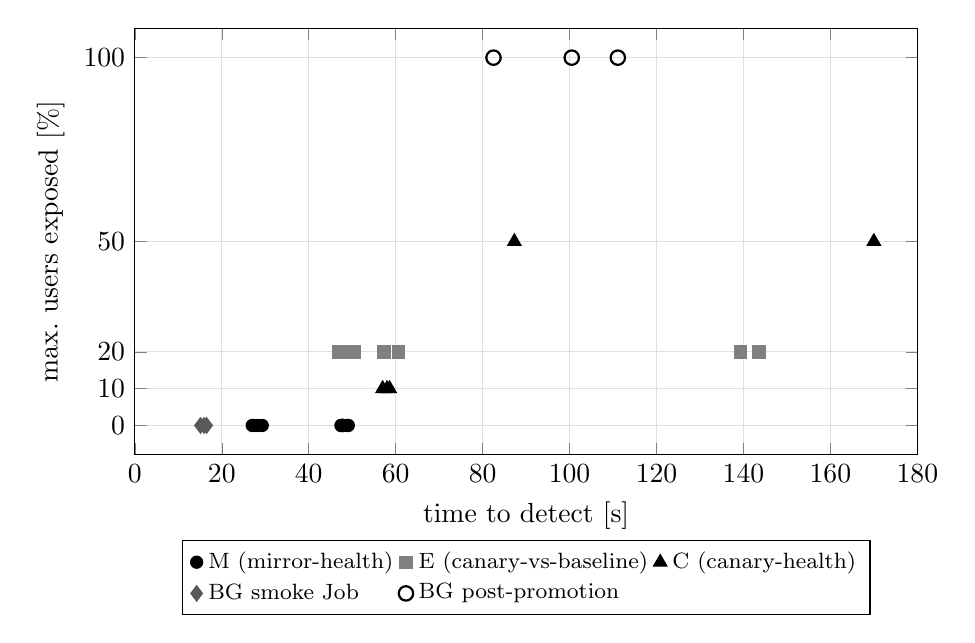
\begin{tikzpicture}
		\begin{axis}[
				width=0.95\textwidth, height=7cm,
				xlabel={time to detect [s]}, ylabel={max.\ users exposed [\%]},
				xmin=0, xmax=180, ymin=-8, ymax=108,
				ytick={0,10,20,50,100},
				grid=major, grid style={gray!25},
				legend style={at={(0.5,-0.2)}, anchor=north, legend columns=3}, legend cell align=left,
				legend style={font=\footnotesize},
			]
			\addplot[only marks, mark=*, mark size=2.2pt, black] coordinates {(28.2,0) (47.5,0) (49.1,0) (27.4,0) (47.8,0) (48.8,0) (27.0,0) (47.9,0) (47.9,0) (29.3,0) (47.7,0) (47.4,0)};
			\addlegendentry{M (mirror-health)}
			\addplot[only marks, mark=square*, mark size=2.2pt, gray] coordinates {(47.4,20) (46.9,20) (49.9,20) (57.3,20) (49.3,20) (50.6,20) (46.9,20) (60.6,20) (139.3,20) (143.6,20)};
			\addlegendentry{E (canary-vs-baseline)}
			\addplot[only marks, mark=triangle*, mark size=2.8pt, black] coordinates {(57.0,10) (58.0,10) (58.6,10) (87.3,50) (170.0,50)};
			\addlegendentry{C (canary-health)}
			\addplot[only marks, mark=diamond*, mark size=2.8pt, gray!70!black] coordinates {(16.5,0) (15.9,0) (15.1,0)};
			\addlegendentry{BG smoke Job}
			\addplot[only marks, mark=o, mark size=2.6pt, thick, black] coordinates {(111.1,100) (100.5,100) (82.5,100)};
			\addlegendentry{BG post-promotion}
		\end{axis}
	\end{tikzpicture}
	\caption{Detected faults F1--F5 and F8 by time to detect and by the highest share of users exposed, one point per run, marked by the check that caught the fault. The points at 139--170\,s are F5 under S4, S6 and S7, counted from the first mirrored request.}
	\label{fig:EvalScatter}
\end{figure}

Recovery was fast in every case: once a check failed, the controller moved all traffic back to the stable version within 0.6--3.2\,s (median 1.8\,s, over the 33 runs caught by a metric or the smoke Job). This time is dominated by the 2\,s polling interval of the runner, so the true recovery time is likely shorter. Rolling back is effectively instant, because the stable version keeps running throughout a canary release; what decides the damage is how long detection takes and how many users are exposed until then.

%----------------------------------------------------------------------------
\subsection{User impact}
\label{sec:EvalImpact}
%----------------------------------------------------------------------------
\autoref{tab:EvalImpact} shows how many user requests reached the faulty version, and how many of them were affected (an error or slower than 500\,ms). Strategies that start with mirroring kept every loud fault away from the users entirely: under S2, S4, S6 and S7, F1, F3 and F4 reached no user. The mirrored copies show what users would have experienced: of the 120--131 copies received during F1, 36--45 failed, about the configured 30\,\%.

\begin{table}[ht]
	\footnotesize
	\centering
	\begin{tabular}{ l r r r r r r r }
		\toprule
		& F1 & F2 & F3 & F4 & F5 & F6 & F8 \\
		\midrule
		\textbf{S0} & 36/10\textsuperscript{p} & 32/2 & 6/6\textsuperscript{p} & 8/4\textsuperscript{p} & 26/0\textsuperscript{p} & 0 & 35/0 \\
		\textbf{S1} C & 21/6 & 189/5 & 23/23 & 17/12 & 90/0 & 0 & 188/0 \\
		\textbf{S2} M & 0 & 38/1 & 0 & 0 & 55/0\textsuperscript{p} & 0 & 75/0 \\
		\textbf{S3} E & 34/16 & 207/3 & 26/26 & 24/17 & 38/0 & 0 & 197/0 \\
		\textbf{S4} M+C & 0 & 204/3 & 0 & 0 & 83/0 & 0 & 244/0 \\
		\textbf{S5} E+C & 42/11 & 332/1 & 27/27 & 30/16 & 54/0 & 0 & 340/0 \\
		\textbf{S6} M+E & 0 & 207/1 & 0 & 0 & 73/0 & 0 & 197/0 \\
		\textbf{S7} M+E+C & 0 & 332/8 & 0 & 0 & 79/0 & 0 & 331/0 \\
		\textbf{BG} & 0 & 0 & 48/48 & 51/31 & 249/0 & 0 & 0 \\
		\bottomrule
	\end{tabular}
	\caption{User requests served by the faulty version / of these, answered with a 5xx code or slower than 500\,ms. \textsuperscript{p}: the version was promoted (in the F2 and F8 columns, every strategy except BG promoted it); the count ends 30\,s after the promotion, after which the fault stays with every user until someone notices it.}
	\label{tab:EvalImpact}
\end{table}

Three results deserve attention.

\paragraph{The experiment exposes more users than the canary.} For the loud faults, S3 and S5 exposed more users than S1: F1 reached 34 and 42 users under S3 and S5 (16 and 11 of them failed), but only 21 under S1 (6 failed). F3 affected 26--27 users instead of 23. This confirms the prediction: the experiment sends 20\,\% of the users to the new version from the start, twice the canary's first step, and it detects in about the same time. Placed before a small canary step, the experiment makes the release less safe for exactly the faults that are easiest to catch.

\paragraph{The experiment is better for slow faults.} For the leak (F5) the order is reversed: the canary caught it only at 50\,\%, after 90 user requests, while the experiment caught it at 20\,\% after 38 (S3) or 54 (S5). The relative memory check needs no long initial delay, because the baseline makes the same start-up allocation as the canary and the difference cancels it out. The canary's absolute check has to wait 90\,s for the start-up allocation to settle, otherwise it would abort healthy releases; by then the canary has reached 50\,\%.

\paragraph{Blue-green trades early safety for late exposure.} The smoke Job caught F1, F2 and F8 before any user was switched, but every fault it does not test for reached all users: F3 slowed down all 48 user requests during the post-promotion analysis, and F5 served 249 user requests before its memory growth was detected. The leak caused no visible errors in this short window, but it would eventually have exhausted the pod's memory.

%----------------------------------------------------------------------------
\subsection{Cost of a healthy release}
\label{sec:EvalCost}
%----------------------------------------------------------------------------
\autoref{tab:EvalCost} and \autoref{fig:EvalCost} show the cost of the healthy release, which every strategy pays on every release, faulty or not. The cost grows with every mechanism: from 11\,s without protection to 6.8 minutes with all three, and from 0.2 to 12.7 pod-minutes. The experiment is the most expensive mechanism: it adds 3.1--3.4 minutes and, because it runs two additional pods, 6.6--8.9 pod-minutes to each release (S0 to S3, S1 to S5, S4 to S7). Mirroring adds 1.4--1.6 minutes and doubles the requests the new version handles during that time (288--334 mirrored copies), which would double the load on its downstream dependencies in a real system.

\begin{table}[ht]
	\footnotesize
	\centering
	\begin{tabular}{ l r r r r }
		\toprule
		& duration [s] & duration [min] & pod-minutes & mirrored or smoke requests \\
		\midrule
		\textbf{S0} & 11 & 0.2 & 0.2 & -- \\
		\textbf{S1} C & 128 & 2.1 & 2.1 & -- \\
		\textbf{S2} M & 97 & 1.6 & 1.9 & 334 mirrored \\
		\textbf{S3} E & 201 & 3.4 & 6.8 & -- \\
		\textbf{S4} M+C & 221 & 3.7 & 4.3 & 294 mirrored \\
		\textbf{S5} E+C & 332 & 5.5 & 11.0 & -- \\
		\textbf{S6} M+E & 299 & 5.0 & 9.4 & 290 mirrored \\
		\textbf{S7} M+E+C & 409 & 6.8 & 12.7 & 288 mirrored \\
		\textbf{BG} & 159 & 2.7 & 2.7 & 50 smoke \\
		\bottomrule
	\end{tabular}
	\caption{Cost of a healthy release (F0): time from start to promotion, and the summed lifetime of the pods created during the trial.}
	\label{tab:EvalCost}
\end{table}

\begin{figure}[ht]
	\centering
	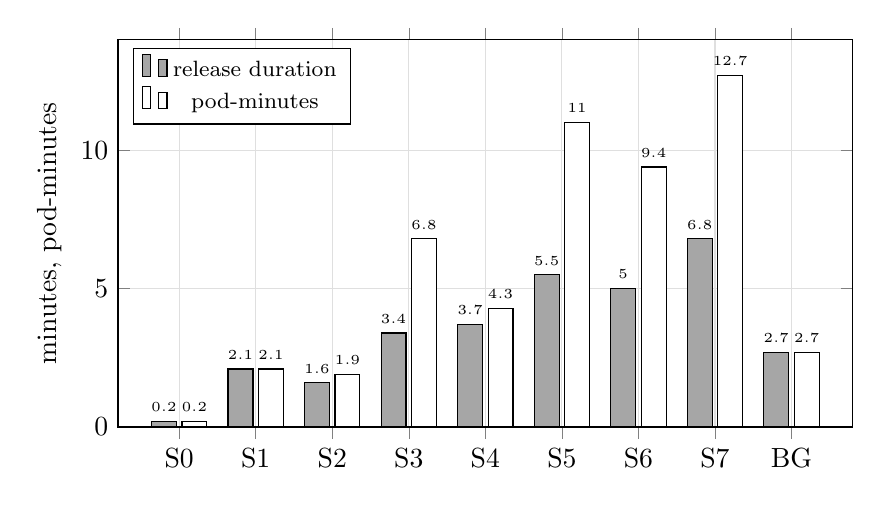
\begin{tikzpicture}
		\begin{axis}[
				ybar, bar width=9pt,
				width=0.9\textwidth, height=6.5cm,
				symbolic x coords={S0,S1,S2,S3,S4,S5,S6,S7,BG},
				xtick=data, ymin=0, ymax=14,
				ylabel={minutes, pod-minutes},
				legend style={at={(0.02,0.98)}, anchor=north west, font=\footnotesize},
				grid=major, grid style={gray!25},
				nodes near coords, nodes near coords style={font=\tiny},
			]
			\addplot[fill=gray!70, draw=black] coordinates {(S0,0.2) (S1,2.1) (S2,1.6) (S3,3.4) (S4,3.7) (S5,5.5) (S6,5.0) (S7,6.8) (BG,2.7)};
			\addlegendentry{release duration}
			\addplot[fill=white, draw=black] coordinates {(S0,0.2) (S1,2.1) (S2,1.9) (S3,6.8) (S4,4.3) (S5,11.0) (S6,9.4) (S7,12.7) (BG,2.7)};
			\addlegendentry{pod-minutes}
		\end{axis}
	\end{tikzpicture}
	\caption{Duration and pod-minutes of a healthy release per strategy.}
	\label{fig:EvalCost}
\end{figure}

The measured durations were close to those estimated in the plan (S1 2.1 minutes against about 2.5, S7 6.8 against about 7.5).

%----------------------------------------------------------------------------
\section{The progress deadline that did not fire}
\label{sec:EvalDeadline}
%----------------------------------------------------------------------------
The progress deadline is the platform's safety net for a version that never starts. It worked in S0--S5 and in BG, but in S6 and S7 the F6 release stayed at step 0 with its pod not Ready, the Rollout reported \emph{Progressing} indefinitely, and nothing happened until the runner aborted it after four minutes. No user was harmed, because a pod that is not Ready receives no traffic. But a release that never ends blocks every later release of the application, and nobody is told: the Rollout does not even become \emph{Degraded}.

%----------------------------------------------------------------------------
\subsection{Observation}
\label{sec:EvalDeadlineObservation}
%----------------------------------------------------------------------------
The two affected strategies have both mirroring and the experiment; the strategies with only one of them (S2, S3, S4, S5) were not affected. Yet in S6 and S7 the F6 release never got beyond the first step, \texttt{setCanaryScale}, so the steps that differ between the strategies had not even started. The cause therefore had to lie in the state the cluster was in \emph{before} the release, not in the release itself.

The state of the ReplicaSets after the matrix gave the decisive clue. The ReplicaSet of the F5 image, scaled to zero replicas, still carried a \texttt{scale-down-deadline} annotation, with a time 30\,s after the abort of the S7--F5 trial, which ran immediately before S7--F6. The controller adds this annotation when it aborts a release, to keep the canary running for \texttt{abortScaleDownDelaySeconds} (30\,s by default) before scaling it down.

%----------------------------------------------------------------------------
\subsection{Root cause}
\label{sec:EvalDeadlineCause}
%----------------------------------------------------------------------------
The source code of the controller~\cite{ArgoRolloutsSource} explains how such an annotation disables the deadline. The deadline is evaluated in \texttt{rollout/sync.go}, but only when the following guard is true:
\begin{lstlisting}[caption={The guard of the progress-deadline check in rollout/sync.go (Argo Rollouts v1.10.1).},label=lst:EvalGuard]
case !isIndefiniteStep(c.rollout) &&
     !isWaitingForReplicaSetScaleDown(c.rollout, c.newRS, c.stableRS, c.allRSs) &&
     conditions.RolloutTimedOut(c.rollout, newStatus):
\end{lstlisting}
The function \texttt{isWaitingForReplicaSetScaleDown} returns true if \emph{any} ReplicaSet of the Rollout, other than the new and the stable one, has a \texttt{scale-down-deadline} annotation. It only checks that the annotation exists, not whether the deadline has passed or whether the ReplicaSet has any replicas left. The intent is reasonable: while an old version is kept running for a delay, the release is not stuck. But a stale annotation keeps the guard false forever, so the deadline is never evaluated.

Three behaviours of the controller combine to leave such a stale annotation behind:
\begin{enumerate}
	\item \textbf{The annotation is added even to an empty ReplicaSet.} When a release is aborted, \texttt{reconcileNewReplicaSet} (\texttt{rollout/replicaset.go}) annotates the canary ReplicaSet as soon as the stable version is fully available. It does not check whether the canary has any replicas to keep.
	\item \textbf{Scaling down during an abort keeps the annotation.} \texttt{scaleReplicaSet} removes the annotation when it scales a ReplicaSet to zero, but not while the Rollout is aborted (\texttt{shouldDelayScaleDownOnAbort} is true).
	\item \textbf{Empty old ReplicaSets are skipped.} After the reset, the aborted ReplicaSet is an old one. \texttt{scaleDownOldReplicaSetsForCanary} (\texttt{rollout/canary.go}) is where old ReplicaSets lose their annotation, by being scaled to zero; but it skips any ReplicaSet that is already at zero replicas.
\end{enumerate}

Whether a release leaves the annotation behind therefore depends on whether the canary ReplicaSet still has replicas when the release is aborted. In S6 and S7, F5 was caught by the experiment. During the experiment step the Rollout's own canary ReplicaSet is at zero, since the canary weight is zero and the experiment runs its own pods. The abort annotated this empty ReplicaSet. The reset 13--14\,s later cleared the abort, and from then on the ReplicaSet was an old, empty one, which nothing ever touched again. In S1 and S4, by contrast, F5 was caught at 50\,\% with the canary pod running. After the reset this ReplicaSet was an old one \emph{with} a replica, so the controller waited for the deadline, scaled it down and removed the annotation, and the following F6 release behaved normally.

The same mechanism explains every F6 result of the matrix:
\begin{itemize}
	\item \textbf{S3 and S5} had the same stale annotation from F5 (caught by the experiment). But F6 starts with the experiment step in these strategies, and it was stopped by the experiment's own deadline, which is evaluated by the experiment controller and does not consult this guard.
	\item \textbf{S2} promoted F5, and \textbf{S0} had no aborted release before F6 at all.
	\item The F1, F3 and F4 ReplicaSets left behind by the experiment in S3 and S5 were cleaned up again before they could matter: the same images were released and aborted by mirroring, with the canary pod running, in S4 and S6.
	\item \textbf{BG} uses a different Rollout, with its own ReplicaSets.
\end{itemize}
Because each fault is always the same image, its ReplicaSet is reused whenever the image is released again, which is how a stale annotation from one trial could reach a later one. In a real system every release has a new image, and the stale ReplicaSet disappears only when it falls out of the revision history, which keeps three old ReplicaSets in this platform and ten by default. Until then, \emph{every} release of the Rollout runs without a working progress deadline.

%----------------------------------------------------------------------------
\subsection{Confirmation}
\label{sec:EvalDeadlineConfirmation}
%----------------------------------------------------------------------------
The analysis makes a prediction that does not depend on mirroring or the experiment at all: as long as the stale annotation exists, F6 should hang under \emph{any} canary strategy, including S1, where it was aborted after 121\,s in the matrix; and once the annotation is removed, the deadline should fire again. Two additional trials, run on 3 November 2026 with the cluster still in the state the matrix had left it in, tested this prediction (\autoref{tab:EvalConfirmation}). Their results were kept apart from the matrix data.

\begin{table}[ht]
	\footnotesize
	\centering
	\begin{tabular}{ l p{4.2cm} l p{5.2cm} }
		\toprule
		Trial & Stale annotation & Predicted & Measured \\
		\midrule
		A: S1 + F6 & present (F5 ReplicaSet, 0 replicas) & hang & no abort; still \emph{Progressing} at step 0 after 232\,s, aborted by the runner \\
		B: S1 + F6 & removed by hand before the release & deadline abort & aborted by the progress deadline after 120.6\,s \\
		\bottomrule
	\end{tabular}
	\caption{Confirmation of the cause of the hang. The only difference between the two trials is the \texttt{scale-down-deadline} annotation on the old, empty F5 ReplicaSet.}
	\label{tab:EvalConfirmation}
\end{table}

Both predictions held. The same strategy and the same image behaved in opposite ways depending only on an annotation on an unrelated, empty ReplicaSet, which confirms that the hang in S6 and S7 was caused by the stale annotation left by the preceding F5 trial, not by the strategies themselves.

%----------------------------------------------------------------------------
\subsection{Relation to known issues and consequences}
\label{sec:EvalDeadlineKnown}
%----------------------------------------------------------------------------
The suppression itself is a known problem. Issue \#4971 of Argo Rollouts~\cite{ArgoRolloutsIssue4971}, opened in August 2026, describes the same guard being kept false by a stale annotation on an orphaned ReplicaSet, which also makes the controller re-queue the Rollout in a tight loop. The pull request proposed to fix it~\cite{ArgoRolloutsPR4972} makes \texttt{isWaitingForReplicaSetScaleDown} ignore deadlines that have already passed; it had not been merged at the time of writing, so v1.10.1 is affected. The issue reproduces the stale annotation differently: the aborted release is left in the aborted state until its scale-down delay expires. The experiments of this work show a second, more ordinary path to the same state, which needs no waiting at all: a release aborted while its own canary ReplicaSet is empty, which is the normal situation during an experiment step, followed by a rollback through Git. A GitOps rollback is the standard reaction to an aborted release, so this path is likely to occur in practice wherever experiment steps are used.

The consequences for the platform are as follows:
\begin{itemize}
	\item The progress deadline cannot be relied on as the only protection against a version that does not start. After an abort in an experiment step, the next releases have no deadline until the stale ReplicaSet leaves the revision history.
	\item The failure is silent: the Rollout stays \emph{Progressing}, so no alert based on the \emph{Degraded} phase fires. An alert on the duration of the \emph{Progressing} phase would catch it.
	\item Until the fix is released, the stale annotation can be removed after an abort (\texttt{kubectl annotate rs <name> scale-down-deadline-}), or the platform can run a periodic job that removes the annotation from ReplicaSets with zero replicas.
\end{itemize}

%----------------------------------------------------------------------------
\section{Discussion}
\label{sec:EvalDiscussion}
%----------------------------------------------------------------------------

\paragraph{RQ1: which mechanism catches what.} Each mechanism has a clear profile. Mirroring catches errors and latency fastest (in 27--49\,s) and without exposing any user, but it is blind to slow faults such as the leak, because its window is short and it measures no memory. The experiment catches every metric fault, the leak included, in 47--61\,s, but it always exposes 20\,\% of the users. The canary also catches every metric fault, but the leak only late and at 50\,\%. None of the metric-based mechanisms can catch a fault below its threshold (F2) or a fault that the metrics do not describe (F8). Only the smoke Job, which checks the content of the responses, caught F8, and it caught F2 only by chance.

\paragraph{RQ2: the cost.} Protection is paid for in time and resources on every release, and the healthy release shows the price. Full protection (S7) takes 6.8 minutes and 12.7 pod-minutes per release, against 2.1 and 2.1 for the canary alone. The experiment accounts for most of the difference. In exposure, the cost is fault-specific: mirroring reduced the users exposed to loud faults to zero, the experiment doubled it, and nothing reduced the exposure to F2 and F8 in a canary release.

\paragraph{RQ3: absolute or relative checks.} In these experiments neither approach produced a false alarm, and both caught the same faults: the relative check was not better at avoiding misses (both missed F2 and F8). The difference was in timing. Because a fresh baseline makes the same start-up allocation as the canary, the relative memory check could start after 60\,s instead of 90\,s, and caught the leak at 20\,\% instead of 50\,\%. The real advantage of relative analysis, robustness against changes of the environment that affect both versions, could not be shown, because environment faults were out of scope. A relative check also has a blind spot of its own: if both versions are bad, for example because of a broken dependency, their difference is small. The absolute checks should therefore stay as a floor.

\paragraph{RQ4: combinations.} Combining mechanisms helps only where a later mechanism catches what an earlier one misses. Mirroring before the canary (S4) moved the loud faults from 10\,\% to 0\,\% exposure, at a cost of 1.6 minutes per release. Adding the experiment to mirroring and canary (S4 to S7) moved the leak from 50\,\% to 20\,\%, for 3.1 more minutes. The canary after mirroring and the experiment (S6 to S7) changed no outcome at all: it only added 1.8 minutes. In the opposite direction, the experiment before a canary (S1 to S5) made the loud faults worse. The order and placement of the mechanisms matter as much as their selection: an experiment placed after the first small canary step, or with a lower weight, would avoid exposing more users than the canary itself.

\paragraph{RQ5: blue-green.} Blue-green inverts the risk profile of the canary. Before the switch it exposes nobody, and a functional smoke test can catch faults that no metric shows (F8). After the switch every user is exposed, and the faults that the smoke test does not cover (latency and the leak) reached all users for 82--111\,s. Its rollback was as fast as the canary's. Blue-green is therefore attractive where a meaningful functional test exists and the faults to be feared are functional ones, and weak against performance faults that appear only under real load.

\paragraph{Defence in depth and a decision guide.} No single mechanism caught every fault, and the strategies that combine complementary mechanisms (mirroring for loud faults, a relative or long-running check for slow ones, a functional test for semantic ones) caught the most with the least exposure. The results suggest the following choices:
\begin{itemize}
	\item a read-heavy service, where users must not see errors: mirroring before the canary (S4);
	\item slow faults expected: add the experiment, but after the first small canary step, not before it;
	\item limited resources or frequent releases: the canary alone (S1);
	\item faults that the metrics cannot see: a functional check, such as the smoke Job, which can also run as an analysis step of a canary;
	\item in every case: an alert on releases that stay \emph{Progressing} too long, because the progress deadline cannot be relied on alone (\autoref{sec:EvalDeadline}).
\end{itemize}

%----------------------------------------------------------------------------
\section{Threats to validity}
\label{sec:EvalThreats}
%----------------------------------------------------------------------------
\paragraph{Internal validity.} Each cell was run once. Most outcomes follow from the configuration (thresholds, delays, step order) and are expected to repeat, which the consistent detection times across strategies support, but the two random outcomes rest on a single sample: F2 under blue-green, caught with a probability of about 64\,\%, and to a lesser extent F4. The trials ran one after the other on the same cluster, and the hang in \autoref{sec:EvalDeadline} shows that state can leak from one trial into the next: the reuse of the same image, and therefore the same ReplicaSet, for every release of a fault made this possible. The other results do not depend on such state, because the metric checks query only the pods of the new version. Four measurement defects were found after the matrix; they affected only the computation of the measurements, which was repeated from the recorded timelines while Prometheus still held the data.

\paragraph{Measurement resolution.} Prometheus scrapes every 10\,s and the checks use one-minute rate windows, so detection times below about 30\,s are not resolved precisely, and the runner's 2\,s polling bounds the resolution of the recovery time.

\paragraph{External validity.} The environment is small: a single node, one replica per version, and synthetic traffic of about 5 requests per second to a single endpoint. With a few requests per measurement window, the checks have little statistical power, and the thresholds were chosen for this application. The faults are deterministic and present from the start, unlike many real faults, which depend on input or appear only under load. Environment faults, where relative analysis is expected to excel, were not tested, and neither were other orders of the mechanisms, such as an experiment after the first canary step. The production environment of the platform was not used.

\paragraph{Future work.} The experiments point to several extensions: statistical canary analysis, which compares canary and baseline with a statistical test instead of fixed thresholds, as Kayenta does~\cite{Kayenta}; testing the experiment after the first canary step and with a lower weight; environment faults; multiple replicas and nodes; and repeated runs of the cells with random outcomes.
